\chapter{Rede de Sensores Sem Fio}
\label{cap:4}

\section{Considerações Iniciais}
A integração de sensores em estruturas, máquinas e ambientes, associada com a entrega eficiente das
informações observadas, pode oferecer inúmeros benefícios para a sociedade, como prevenção de catástrofes,
conservação de recursos naturais e aprimoramento de comodidade e segurança. Isso pode ser alcançado através
da implantação de uma rede de sensores sem fio (RSSF) \cite{townsend_arms2005}.

Uma RSSF pode ser definida como uma rede de dispositivos, denominados nós, que podem monitorar o ambiente e
comunicar a informação adquirida através de ligações sem fio. Esses dados são transmitidos, diretamente ou por
múltiplos saltos, dependendo da topologia da rede, para um dispositivo principal, que pode estar conectacdo à
outras redes, como a \textit{Internet}, e que oferece uma interface de interação entre o usuário e a RSSF
\cite{buratti2011}.

Quanto à sua aplicação em um sistema de automação residencial, de acordo com os princípios mencionados no
Capítulo \ref{cap:2}, ela torna-se parte integrante da rede de controle, pois atua apenas sobre os sensores e
atuadores e não sobre os aparelhos de consumo e possibilita com que o residente a gerencie através de um
dispositivo de controle remoto.

Para \cite{townsend_arms2005}, a RSSF ideal deve ser escalável, consumir muito pouca energia, ter capacidade
de rápida aquisição de dados, ser confiável e precisa a longo prazo, possuir baixo custo de desenvolvimento e
instalação e não necessitar manutenção significativa.

Em relação à sua implementação, alguns aspectos importantes devem ser definidos antes do processo de
desenvolvimento, sendo eles a composição dos nós, a topologia da rede e os mecanismos de segurança.

\section{Composição dos Nós}
Os nós de uma RSSF são compostos de cinco componentes principais, sende eles uma unidade controladora, um
dispositivo de armazenamento de memória, sensores e atuadores, um transceptor sem fio e uma fonte de energia.
Cada um desses componentes deve operar seguindo um equilíbrio entre o menor consumo de energia possível e a
necessidade de cumprir suas tarefas \cite{karl_willig2005}.

Na prática, a unidade controladora e o armazenamento de memória tornam-se um só componente com o uso de
microcontroladores, ou MCU (\textit{Microcontroller Unit}), para cumprir tais funções. Desse modo, a
composição de um nó de uma RSSF é normalmente conforme ilustrado na figura \ref{figura:node}.

\begin{figure}[h]
	\caption{Composição de um nó em uma RSSF}
	\centering
	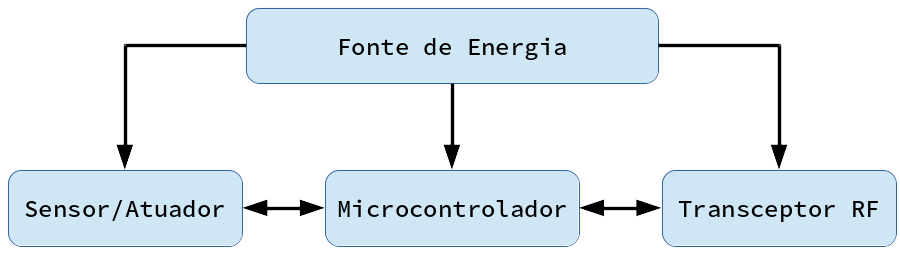
\includegraphics[scale=0.5]{../images/node.png}
	\hspace{\linewidth}
	Fonte: elaborada pelo autor
	\label{figura:node}
\end{figure}

\subsubsection{Microcontrolador}

